\documentclass[12pt]{report}

\usepackage[T1]{fontenc}
\usepackage[utf8]{inputenc}
\usepackage{graphicx}

\begin{document}
 
\begin{center}
{\Huge Dieño del puente H}
\end{center}
\begin{center}

\includegraphics[scale=1]{../../../../Downloads/upzmg.jpg} 
\end{center} 
{\Huge Enesto Alonso Partida López\\Osmar de Jesus Cruz Ramirez\\ Universidad Politecnica De La Zona Metropolitana De Guadalajara\\ Mecatronica 4 A\\ Septiembre-diciembre 2019}
\date{25 de octubre 2019}
 
\newpage

{\huge \textbf{INTRODUCCION:}\\}\\


{\large medinate la utilizacion de un cicuito conocido como el puente H (esto debido a su forma al conectarse), sera necesario hacer girar un motor de vajo voltaje hacia un lado y posteriormente haci ael otro esto mediante la activacion de relevadores, para lo cual se utilizar un arduiono que tenga la programacoion para lograr que el motor gire a ambos lados dependiendo de la polarizacion que se le otorge}\\
 

{\huge \textbf{OBJETIVO}\\}\\


{\large lograr que el motor gire hacia ambos lados esto dependiendo de la polarizacion que se le otorgue esto mediante un boton que permita el paso de corriente}\\



{\huge \textbf{MARCO TEORICO}\\}\\


{\large El puente H  es un circuito electrónico que permite a un motor eléctrico DC girar en ambos sentidos, avanzar y retrocerder.
Los puentes H ya vienen hechos en algunos circuitos integrados, pero también se pueden construir a partir de componentes eléctricos y/o electronicos.
Un puente H se construye con 4 interruptores (mécanicos o mediante transistores). Cuandos los interruptores S1 y S4 están cerrados ( S2 y S3 abiertos ) se aplica una tensión haciendo girar el motor en un sentido. Abriendo los interruptores S1 y S4 ( cerrando S2 y S3 ), el voltaje se invierte, permitiendo el giro en sentido inverso del motor.Un puente H no solo se usa para invertir el giro de un motor, también se puede usar para frenarlo de manera brusca, al hacer un corto entre los bornes del motor, o incluso puede usarse para permitir que el motor frene bajo su propia inercia, cuando desconectamos el motor de la fuente que lo alimenta.\\}\\
\begin{center}
\begin{figure}[hbtp]
\caption{Diagrama del puente H}
\centering
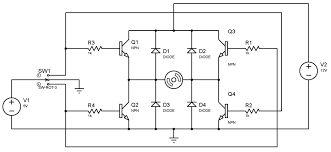
\includegraphics[scale=1]{../../../../Downloads/descragas/descarga.png}
\end{figure}

\end{center}


{\huge \textbf{MATERIALES}\\}\\


\begin{enumerate}
\item Protoboard
\item Placa de arduino
\item Relevadores
\item Resistencias
\item Optoacopladores
\item 2N2222
\item Fuente de Voltaje
\item Leds
\item Push Botton
\item Clabe Para Protoboard
\item Caimanes
\item Transistores o MOSFET
\item Motor de 5v -12v
\end{enumerate}


{\huge \textbf{Desarrollo}\\}\\
\begin{enumerate}
\item Se comenzará con el armado del circuito que consta de dos push botton, los cuales cada botton van acoplados a un optoacoplador (4N25) el cual será el que emita la señal a la placa Arduino la cual ira conectado a los transistores 2N2222 los cuales posteriormente irán conectados a los relevadores que se accionaran a presionar el botón, un extra, será agregar un led el cual indique cuando ente en funcionamiento el relevador. Cabe de resaltar que la programacion del arduino sera la misma
\item cuando se tiene armado el circuito con los relevadores que se accionaran al precionar los botones sera necesario armar el puente H, en esta caso se utilizaran los trasnsistores IRF640N, los cuales cuentan con un diodo rectificador el cual ya no sera necesario colocar en el armado del circuito, el circuito debera ser como el siguiente(figura 2):
\begin{center}
\begin{figure}[hbtp]
\centering
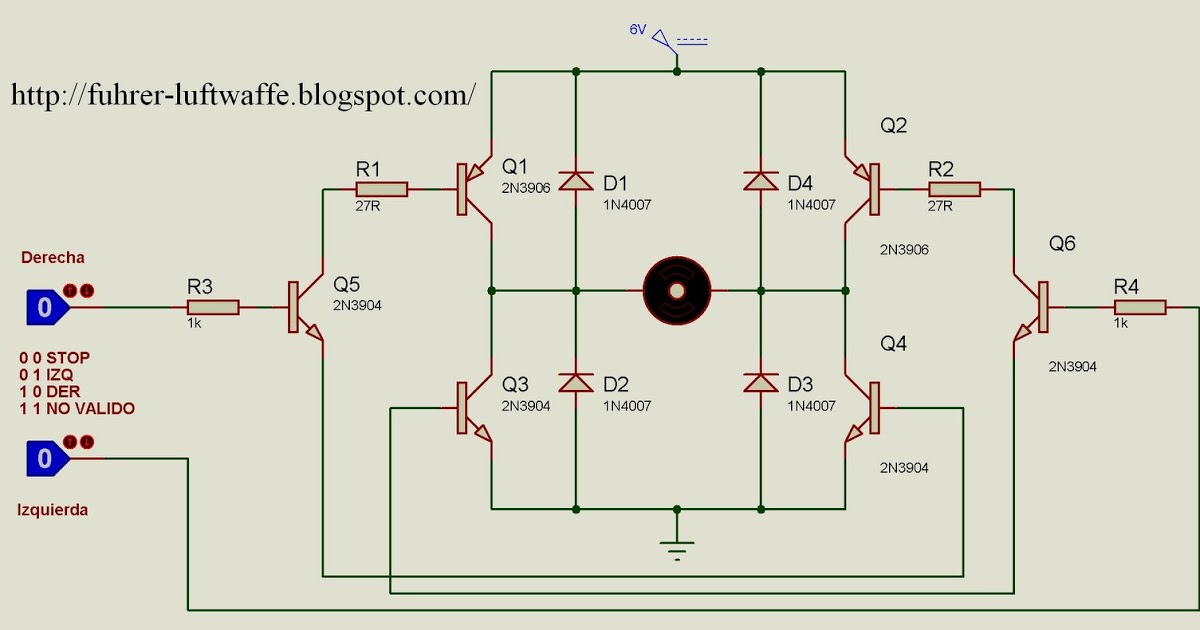
\includegraphics[scale=0.2]{../../../../Downloads/descragas/puente.jpg}
\caption{Diagrama del puente H}
\end{figure}
\end{center}
\item cuando se hallan realizado los dos circuito sera necesario conectarlos, para esto, se remplazaran los botones que se tenian en el puente H y se sustinuiran por una coneccion proveniente de los relevadores, uno para cada boton, esto nos permitira accionar el motor, dependiendo del relevedor activado el motor debera girar hacia un lado y activando el otro el mortor devera girar al lado contrario
\item se tiene que tener cuidado de no accionar el motor hacia un lado e inmediatamente hacia el lado contario porque puede provocar que el motor sufra una falla y deje de funcionar.
\end{enumerate}

{\huge \textbf{Resultados obtenidos}\\}\\
{\large Esta fue nuestra primera operacion para calcular el primer valor de nuestra
resistencia que viene despues del push button:\\
R = 12 V/ 80mA = 150 ohm\\
la segunda operacion para calcular nuestra segunda resistencia que esta colocada
en la salida de nuestro arduino utilizamos la siguiente operacion:\\
R = (Vin - 0.6) (HFE)/12 A.\\
El HFE lo obtuvimos mediante la medidcion del 2N2222A. en un multimetro
con entrada para la medicion de transistores. asi fue como conocimos el valor
de nuestro 2N2222A.\\
el cual fue nuestra operacion: R= (12 v - 0.6)(250 HFE) / 12 A= 3950}\\
posteriormente se logro realizar el objetivo de la practica, aunque no estetico fue gratificante ver que el motor giraba en centido de las manecillas del reloj y posteriormente encontra de las mismas y el circuito quedo de la siguiente manera:
\begin{center}
 \begin{figure}[hbtp]
 \centering
 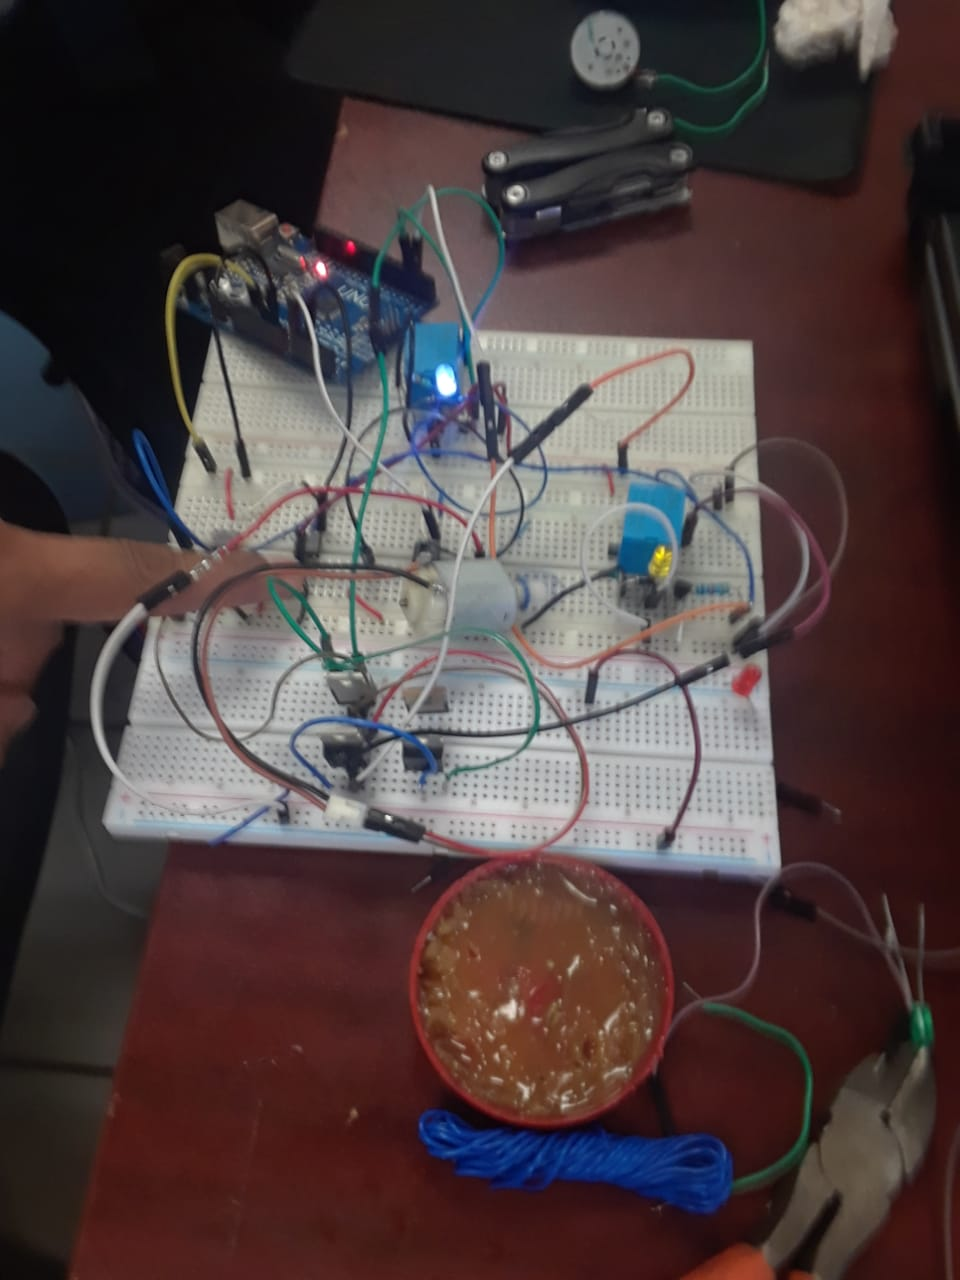
\includegraphics[scale=0.45]{circuito.jpeg}
 \caption{Circuito terminado}
 \end{figure}
 \newpage
 \end{center} 
{\huge \textbf{Conclusión}\\}\\
{\large Como previamente se conoció el actuar de los 2N2222 y los optoacopladores 4N25 fue más fácil entender como funcionaria el circuito, en este caso el problema principal fue que, al realizar el puente H en ocasiones solo conducía energía por un solo lado del circuito y por lo tanto el motor solo giraba en dirección de las manecillas del reloj y no encontra de las mismas, más sin embargo se logró resolver después de un riguroso análisis de las conexiones y encontrar que las conexiones se encontraban mal lo cual no permitía el paso de la corriente para lograr accionar el motor pero se logró el objetivo de hacer que el motor girar en ambos sentidos solo con activar un relevador.}
\newpage
{\huge \textbf{Bibliografia:}\\}\\
@online{Electronica Unicrom,
author = {Frank Mecafenix },
title = {Ingeniería Mecafenix},
year = {2016},
url = {https://www.ingmecafenix.com/electronica/puente-h-control-motores/},
OPTsubtitle = {La enciclopedia de la ingeniería},
OPTlanguage = {Español},
OPTversion = {1},
OPTdate = {21},
OPTmonth = {6},
OPTurldate = {https://www.ingmecafenix.com/electronica/puente-h-control-motores/},
}


\end{document}